\documentclass[12pt]{article}
\usepackage[margin=1in]{geometry}
\usepackage[section]{placeins}


\usepackage{fancyhdr}
\pagestyle{fancy}
\rhead{\thepage}
\fancyfoot{}

\usepackage{graphicx}
\graphicspath{ {./assets/images/} }

\usepackage{xcolor}
\usepackage{listings}

\begin{document}

% \title{Man in the Middle}
% \author{Enan Ajmain}
% \maketitle

\begin{titlepage}
    \begin{center}
        \line(1,0){400} \\
        [0.25in]
        \huge{\bfseries ARP Poisoning} \\
        \huge{\bfseries and} \\
        \huge{\bfseries Man in the Middle Attack} \\
        [2mm]
        \line(1,0){400}\\
        [2cm]
        \textsc{\Large A report on the MitM attack} \\
        [2cm]
        \textsc{\small by} \\
        \textsc{\large Nafid Ajmain Enan} \\
        \textsc{\large 1605018} \\
        \textsc{\large Group 9} \\
    \end{center}

\end{titlepage}

\section{Introduction}

Man in the Middle is a cyberattack where the attacker secretly sniffs, relays,
and possibly alters the packets exchanged between two parties. The parties
believe they are directly communicating with each other, while the attacker sits
in the middle and observes their communication.

\vspace{1cm}

\begin{figure}[h]
    \centering
    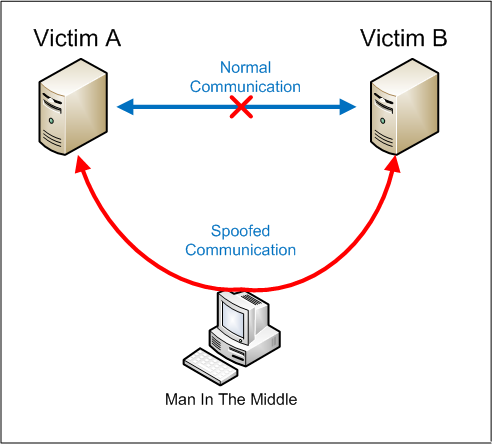
\includegraphics[scale=0.75]{topology}
    \caption{Topology of Man-in-the-Middle attack}
\end{figure}

\FloatBarrier

\vspace{1cm}

\section{Steps of Attack}

To demonstrate the attack I configured three docker containers. Two of them ---
Host A and Host B --- are the victims and one --- Host M --- is the attacker.

\vspace{1cm}

\begin{table}[h!]
    \centering
    \begin{tabular}{ |c|c|c| }
        \hline
        Host Name & IP Address & MAC Address \\
        \hline
        \hline
        Host A & 10.9.0.5 & 02:42:0a:09:00:05 \\
        \hline
        Host B & 10.9.0.6 & 02:42:0a:09:00:06 \\
        \hline
        Host M & 10.9.0.105 & 02:42:0a:09:00:69 \\
        \hline
    \end{tabular}
    \caption{IP and MAC addresses of the hosts}
\end{table}

\vspace{1cm}

\subsection{Setting up the communication}

After setting up the hosts, I set up a communication between the victim hosts
with a ping command.

\vspace{1cm}

\begin{lstlisting}[language=bash,caption={Shell commands},captionpos=b]
# At Host A
ping 10.9.0.6

# At Host B
tcpdump -i eth0 -n icmp
\end{lstlisting}

\vspace{1cm}

The figure below demonstrates a ICMP communication between hosts A and B. Host A
sends the ICMP ping echo requests and B sends the replies.

\begin{figure}[h]
    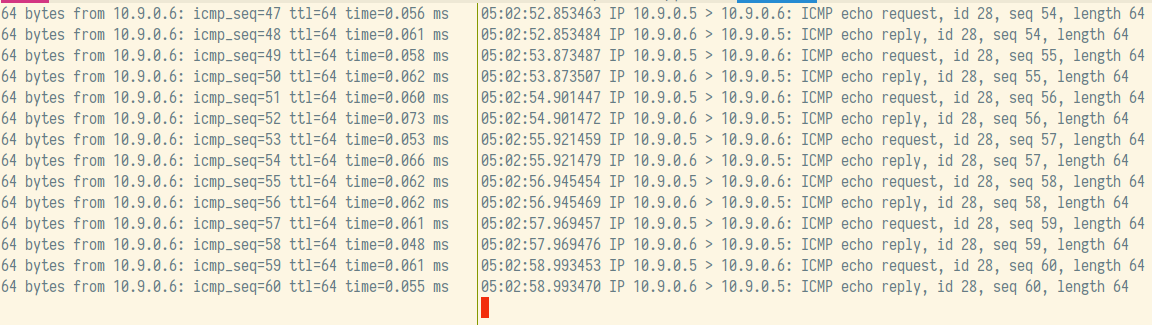
\includegraphics[scale=0.4]{normal-icmp}
    \caption{Normal ICMP communication}
\end{figure}

\FloatBarrier

\vspace{1cm}

\subsection{ARP Poisoning}

Now that a communication is in place between the victim hostws, we need to
poison their ARP caches. After building my project, we can begin poisoning the
caches with the following command.

\vspace{1cm}

\begin{lstlisting}[language=bash,caption={Begin ARP poisoning},captionpos=b]
# At Host M
# binary_file   Host A   Host B   Interface
./spoofer/spoof 10.9.0.5 10.9.0.6 eth0
\end{lstlisting}

\vspace{1cm}

The binary will begin poisoning the ARP caches of both the victim hosts
continuously. Continuously because if the attacker stops poisoning the caches,
the victim hosts will reset their caches with correct entries.

\vspace{1cm}

\begin{lstlisting}[language=bash,caption={Before and after ARP poisoning},captionpos=b]
# At Host A, before being poisoned
Address       HWtype  HWaddress           Flags Mask  Iface
10.9.0.6      ether   02:42:0a:09:00:06   C           eth0
10.9.0.105    ether   02:42:0a:09:00:69   C           eth0

# At Host B, before being poisoned
Address       HWtype  HWaddress           Flags Mask  Iface
10.9.0.5      ether   02:42:0a:09:00:05   C           eth0
10.9.0.105    ether   02:42:0a:09:00:69   C           eth0

# At Host A, after being poisoned
Address       HWtype  HWaddress           Flags Mask  Iface
10.9.0.6      ether   02:42:0a:09:00:69   C           eth0
10.9.0.105    ether   02:42:0a:09:00:69   C           eth0

# At Host B, after being poisoned
Address       HWtype  HWaddress           Flags Mask  Iface
10.9.0.5      ether   02:42:0a:09:00:69   C           eth0
10.9.0.105    ether   02:42:0a:09:00:69   C           eth0
\end{lstlisting}

\vspace{1cm}

From the figure above we see that the ARP caches of hosts A and B are poisoned
since the entries to each other's MAC address point to host M. Now any packet
host A sends to B or B to A, it will go to M instead. That's why, after the ARP
caches are poisoned you'll see the ICMP communication between hosts A and B halt
without error or warning. It's because they cannot find each other anymore.

\vspace{1cm}

\subsection{Man in the Middle Attack}

Now that we've successfully poisoned the ARP caches of the victim hosts, we'll
need to sniff the incoming packets and relay them back to their intended target,
so that the victims will not know they have been attacked.

Before launching the sniffer, remember to turn IP forwarding off. Normally,
you'd turn it on because it would automatically relay the sniffed packets to
their target, but that will also send an additional ARP reply with actual MAC
addresses of the hosts which will clash with our ARP spoofing. So, we'll have to
relay the packets ourselves.

\vspace{1cm}

\begin{lstlisting}[language=bash,caption={Ip fowarding},captionpos=b]
# Turn IP forwarding off
sysctl net.ipv4.ip_forward=0

# Turn IP forwarding on
sysctl net.ipv4.ip_forward=1
\end{lstlisting}

\vspace{1cm}

After turning the IP forwarding off, you can now launch the sniffer, which will
sniff the packets and log them down in a file named \verb|snifflog| and then
relay the packets to their intended target.

{\bf Note:} The sniffer doesn't take input. It reads the IP and MAC addresses of
the hosts and the network interface from a file generated by the \verb|spoofer|.

\vspace{1cm}
\begin{lstlisting}[language=bash,caption={Start sniffing},captionpos=b]
./sniffer/sniff
\end{lstlisting}
\vspace{1cm}

After the sniff and relay binary is successfully launched, the halted
communication between hosts A and B will resume. The packets exchanged between
them will go through host M who is sniffing the packets before relaying them to
their originally intended target.

\vspace{1cm}
\begin{figure}[h]
    \centering
    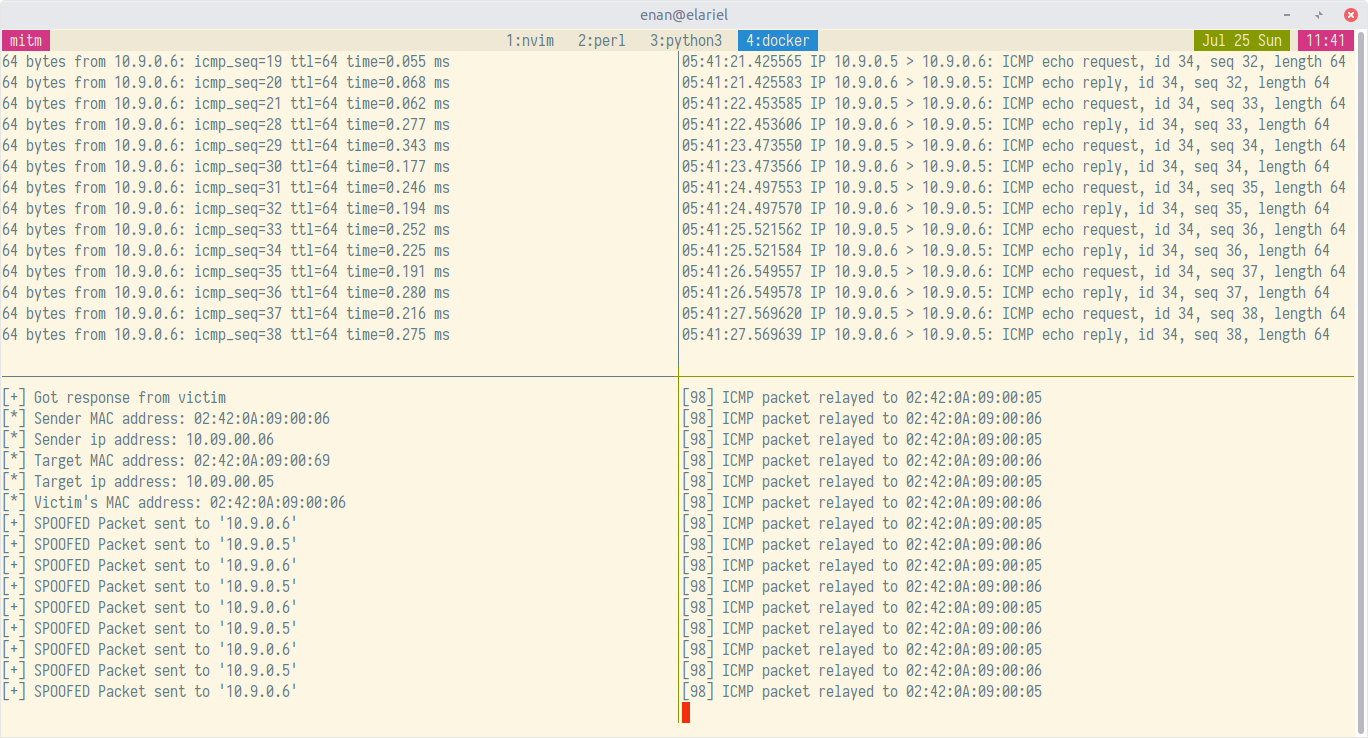
\includegraphics[scale=0.3]{breached-icmp}
    \caption{Breached ICMP communication}
\end{figure}

\FloatBarrier

\vspace{1cm}
\subsection{TCP Protocol}

MitM attack can be launched in TCP protocol as well. To set up a TCP
communication between hosts A and B we can use \verb|netcat| as follows.

\vspace{1cm}
\begin{lstlisting}[language=bash,caption={Start TCP communication},captionpos=b]
# On Host B (server)
nc -lp 9090

# On Host A (client)
nc 10.9.0.6 9090
\end{lstlisting}
\vspace{1cm}

After the TCP communication is set up, the rest of the procedure is the same.
Launch the ARP spoofer binary and the sniffer binary and the packets exchanged
between hosts A and B will go through host M as it sniffs and relays the packets
to their intended targets.

\section{Countermeasure}

By the nature of how ARP caching works, it is nearly impossible to prevent ARP
poisoning. The only sure way to prevent it is to use static ARP cache. But this
method is not feasible in real-life usage.

The other way to prevent man-in-the-middle attack is to encrypt the packets
being exchanged, so that even if an attacker could get hold of the packages they
could not decipher it. What needs to be noted, though, is that if the key for
the encryption should not be sent through an unsecured communication, because
the attacker might intercept the key as well, which will render the whole
concept of encryption ineffectual.


\end{document}
